\section{Experiments}
\vspace{-1ex}
\label{section:experiments}

For conciseness, several experiments are relegated in appendix: 

\begin{enumerate}
    \item \textbf{TS-LDDMM representation identifiability, \Cref{appendix: identifiability}:} On synthetic data, we evaluate the ability of our method to retrieve the parameter $v_0^*$ that encodes the deformation $\varphi^{\{v_0^*\}}$ acting on a time series graph $\msg$ by solving the geodesic shooting problem \eqref{eq:relaxation} between $\msg$ and $\varphi^{\{v_0^*\}}.\msg$.
     \textbf{Results} show that TS-LDDMM representations are identifiable or weakly identifiable depending on the velocity field kernel $K_G$ specification.
  
    \item \textbf{Robustness to irregular sampling, \Cref{appendix: robustness}:} We compare the robustness of TS-LDDMM representation with 9 URL methods handling irregularly sampled multivariate time series on 15 shape-based datasets (7 univariates \& 8 multivariates).
     We assess methods' classification performances under regular sampling (0\% missing rate) and three irregular sampling regimes (30\%, 50\%, and 70\% missing rates), according to the protocol depicted in \cite{kidger2020neural}.
      \textbf{Results} show that our method, TS-LDDMM, outperforms all methods for sampling regimes with missing rates: 0\%, 30\%, and 50\%.
      %{\color{red} J'enlèverai cette phrase ou je développerai en Appendix : The performance decrease of the Kernel-SVC based on TS-LDDMM representation is sensibly due to the misspecification of its regularization parameter.}
    
    \item \textbf{Classification benchmark on regularly sampled datasets, \Cref{appendix: shape_classification}:} We compare performances of a kernel support vector machine (SVC) algorithm based on TS-LDDMM representation with 3 state-of-the-art classification methods from shape analysis on 15 shape-based datasets (7 univariates \& 8 multivariates). \textbf{Results} show that the TS-LDDMM-based method outperforms other methods (best performances over 13 datasets), making TS-LDDMM representation relevant for time series shape analysis.
\end{enumerate}
\begin{figure*}[t]
  \centering
  \begin{subfigure}[b]{0.49\textwidth}
    \centering
    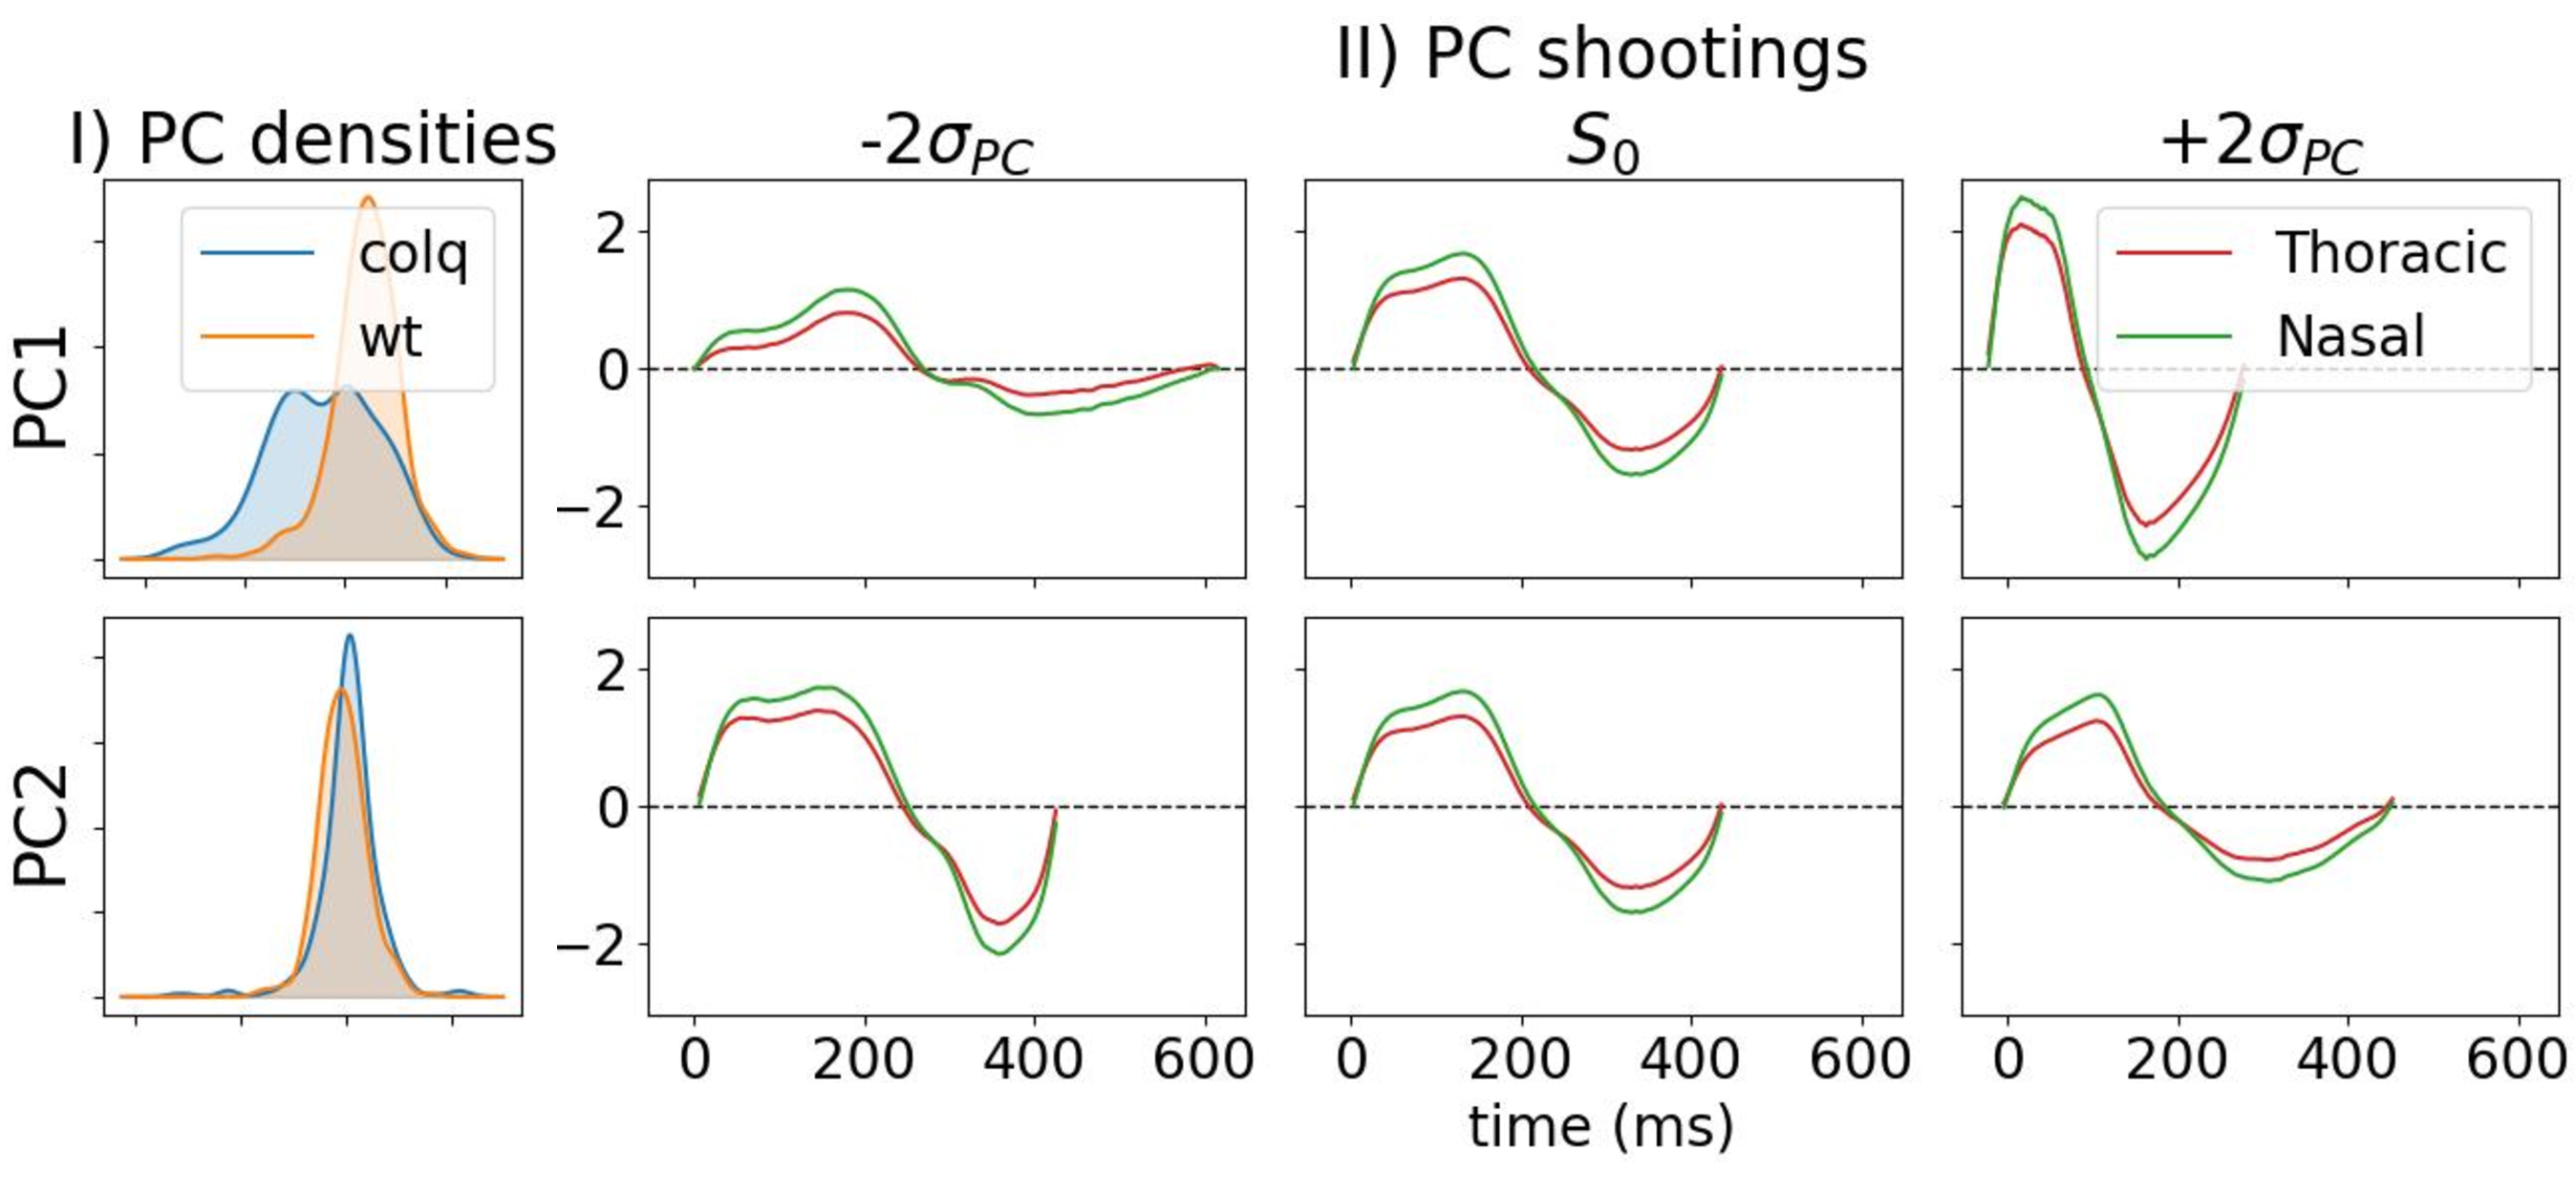
\includegraphics[width = \textwidth]{pictures/ts_ddmm_shooting.pdf}
    \caption{TS-LDDMM}
    \label{fig:ts-lddmm shooting}
  \end{subfigure}
  \begin{subfigure}[b]{0.49\textwidth}
    \centering
    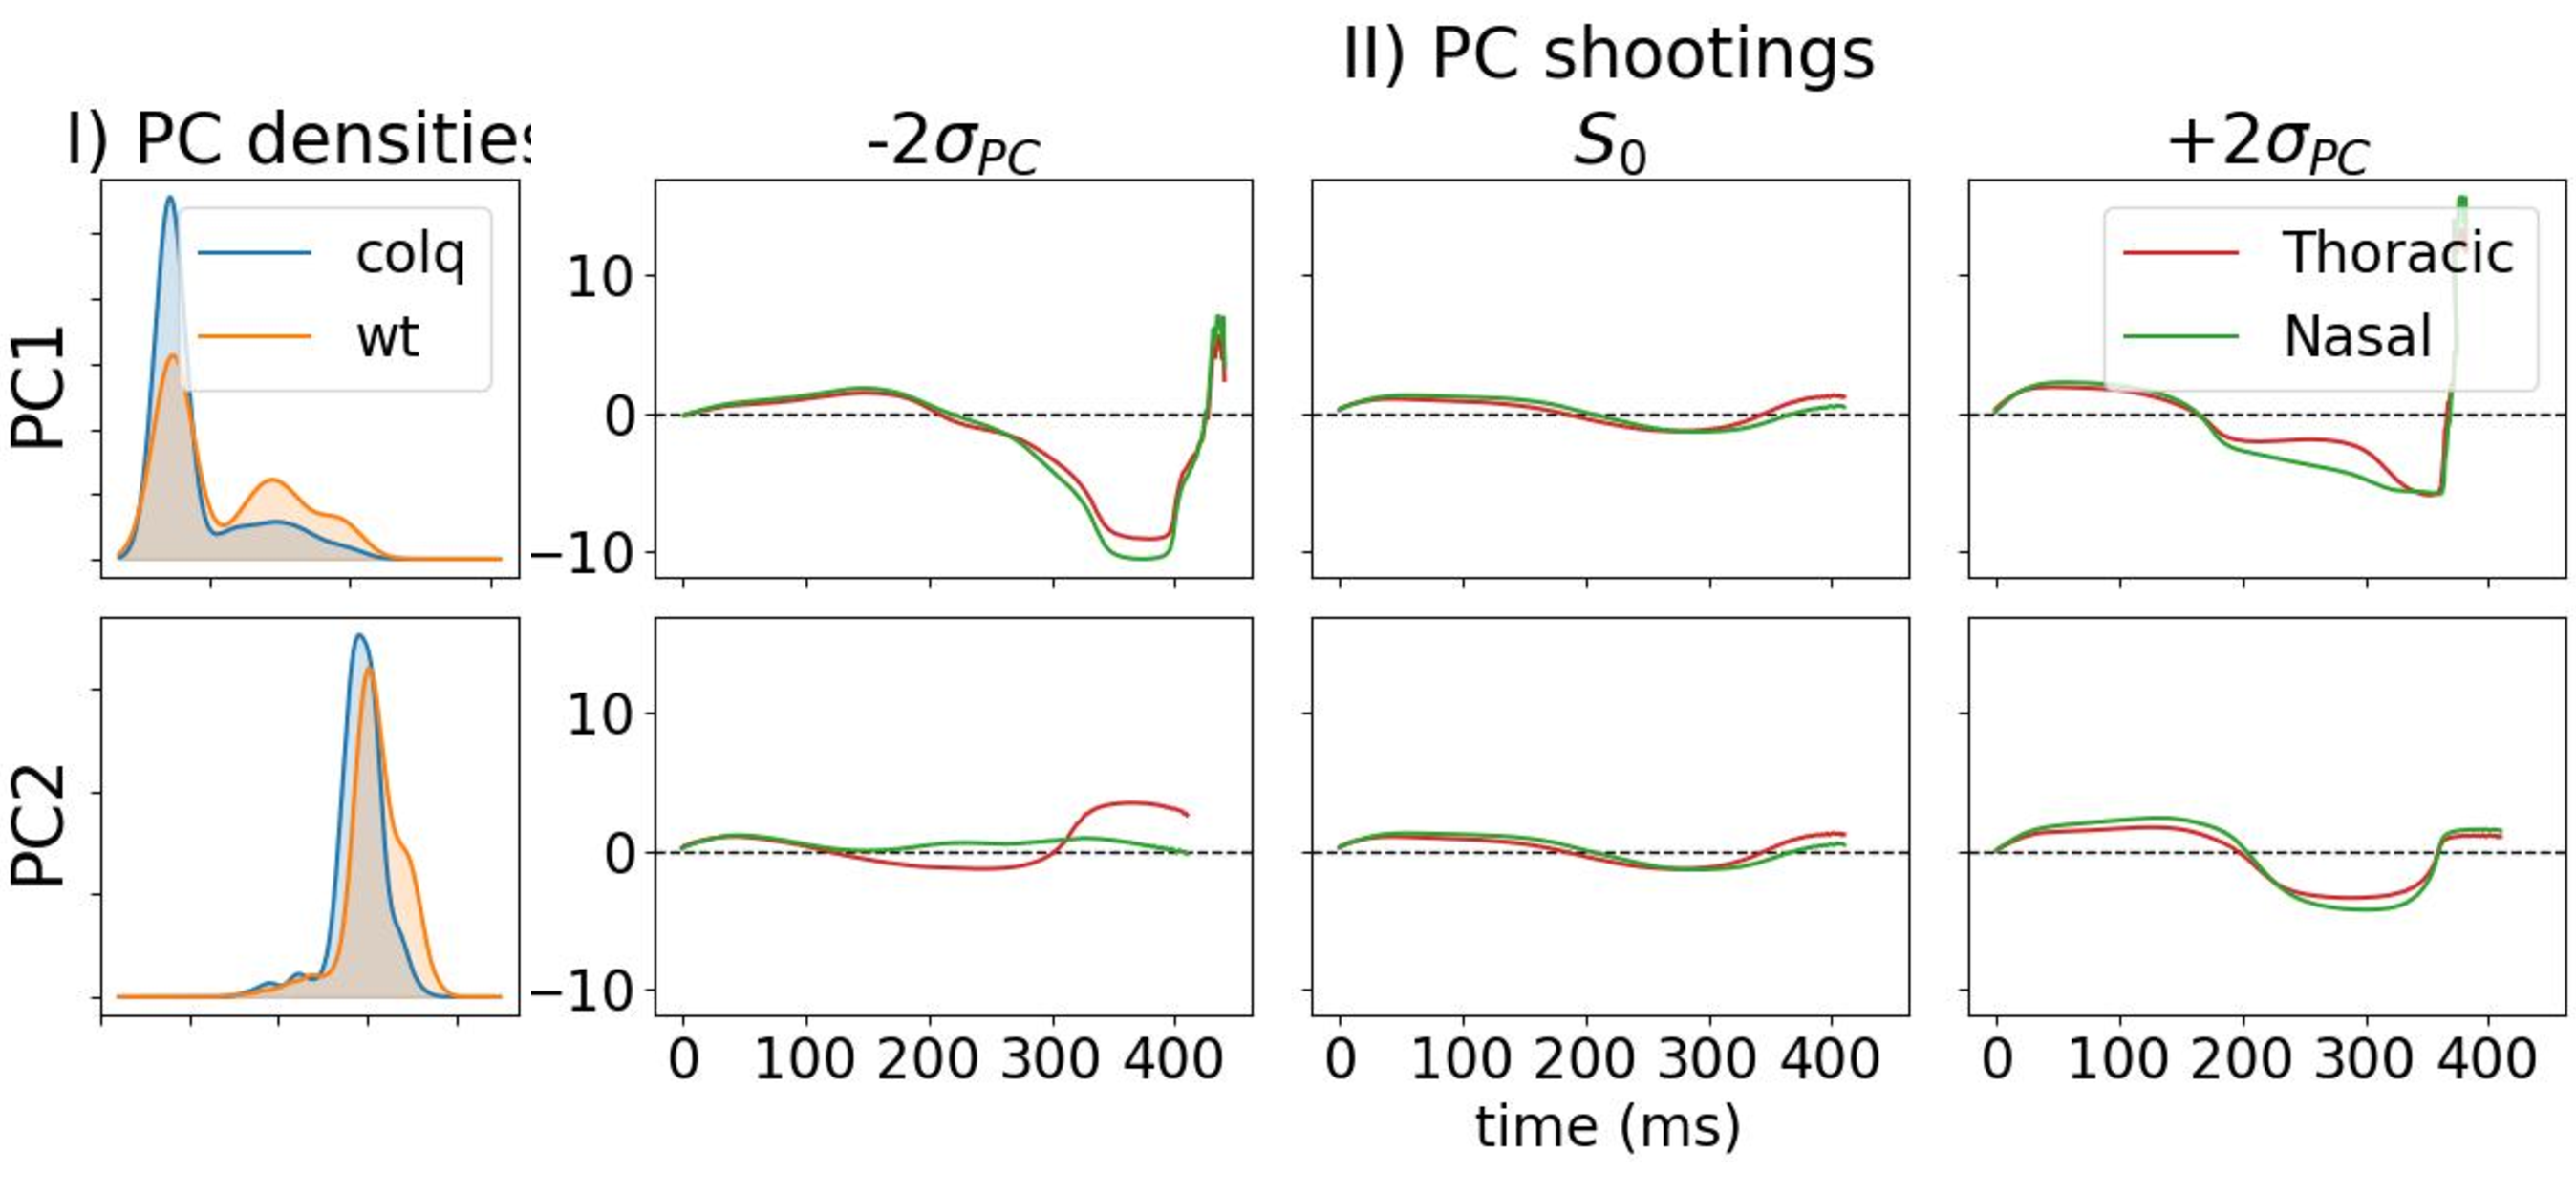
\includegraphics[width = \textwidth]{pictures/lddmm_shooting.pdf}
    \caption{LDDMM}
    \label{fig:lddmm shooting}
  \end{subfigure}
  \caption{Analysis of the two principal components (PC) related to mice' respiratory cycles before exposure for TS-LDDMM \Cref{fig:ts-lddmm shooting}, and LDDMM \Cref{fig:lddmm shooting}.
  In both cases, I) displays PC densities according to mice genotype and II) displays  deformations of the reference graph $S_0$ along each PC.}
  \label{fig:exp1}
\end{figure*}

\vspace{-1ex}
\begin{figure*}[t]
  \centering
  \begin{subfigure}[b]{0.15\textwidth}
    \centering
    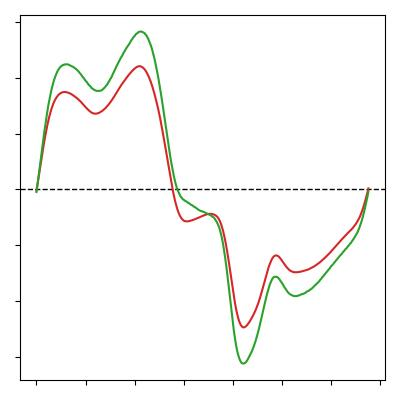
\includegraphics[width = \textwidth]{pictures/exp_1_cycle_example.jpeg}
    \caption{colq cycle}
    \label{fig:colq-cycle}
  \end{subfigure}
  \begin{subfigure}[b]{0.15\textwidth}
    \centering
    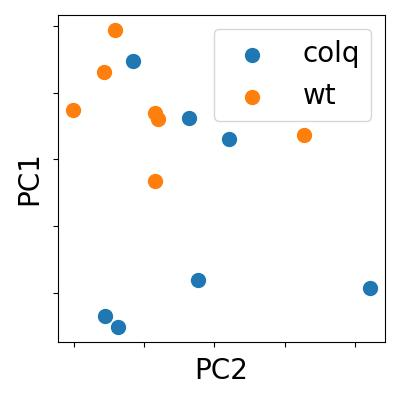
\includegraphics[width = \textwidth]{pictures/exp_1_scatter.jpeg}
    \caption{PC1 vs PC2}
    \label{fig: pcs-scatter}
  \end{subfigure}
  \begin{subfigure}[b]{0.15\textwidth}
    \centering
    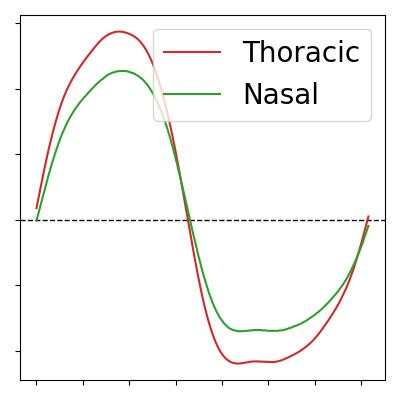
\includegraphics[width = \textwidth]{pictures/exp_1_wt.jpeg}
    \caption{wt cycle}
    \label{fig:wt-reference}
  \end{subfigure}
  \caption{\Cref{fig:colq-cycle} is a \textbf{colq} respiratory cycle. \Cref*{fig: pcs-scatter} displays individual mouse reference respiratory cycle in the TS-LDDMM PC1-PC2 coordinates. \Cref{fig:wt-reference} is a referent respiratory cycle of a \textbf{wt} mouse learned with TS-LDDMM. }
  \vspace{-1em}
\end{figure*}
\vspace{-1ex}
\subsection{Interpretability: analysis of respiratory behavior in mice}
\label{section:interpretability}
\vspace{-1ex}
%We consider a dataset composed of mouse respiratory time series before and after a drug injection.
% A complete presentation of this dataset is given in \Cref{appendix:mouse_dataset}.
%  The mouse are divided in two groups depending on their genotypes : \textit{colq} and \textit{wt}.
%  We aim to study the difference of respiratory shapes according to the genotype.
%   That is why, TS-LDDMM \eqref{eq:general_optimization_problem} is applied to derive the features representations $(\mathbf{\alpha}_j)_{j\in[N]}\in (\Rset^2)^N$ related to $N$=\sam{fill} respiratory time series coming from 14 mouse (7 \textit{colq} and \textit{wt}) before drug injection.
%   Then, a Principal Components Analysis (PCA) is performed on $(\mathbf{\alpha}_j)_{j\in[N]}$





%the densities of each genotype according to each PC are displayed. In Figure B), the deformations of the reference graph $S_0$ along each PC are given. In Figure D), the graph of reference $S^j$, also called barycenter, related to each mouse, is displayed according to their coordinates on PC1 and PC3. In Figure C) et E), illustrations of respiratory cycles related to mice coming from the \textbf{wt} and \textbf{colq} group are displayed.

%\begin{figure*}[t]
%  \centering
%  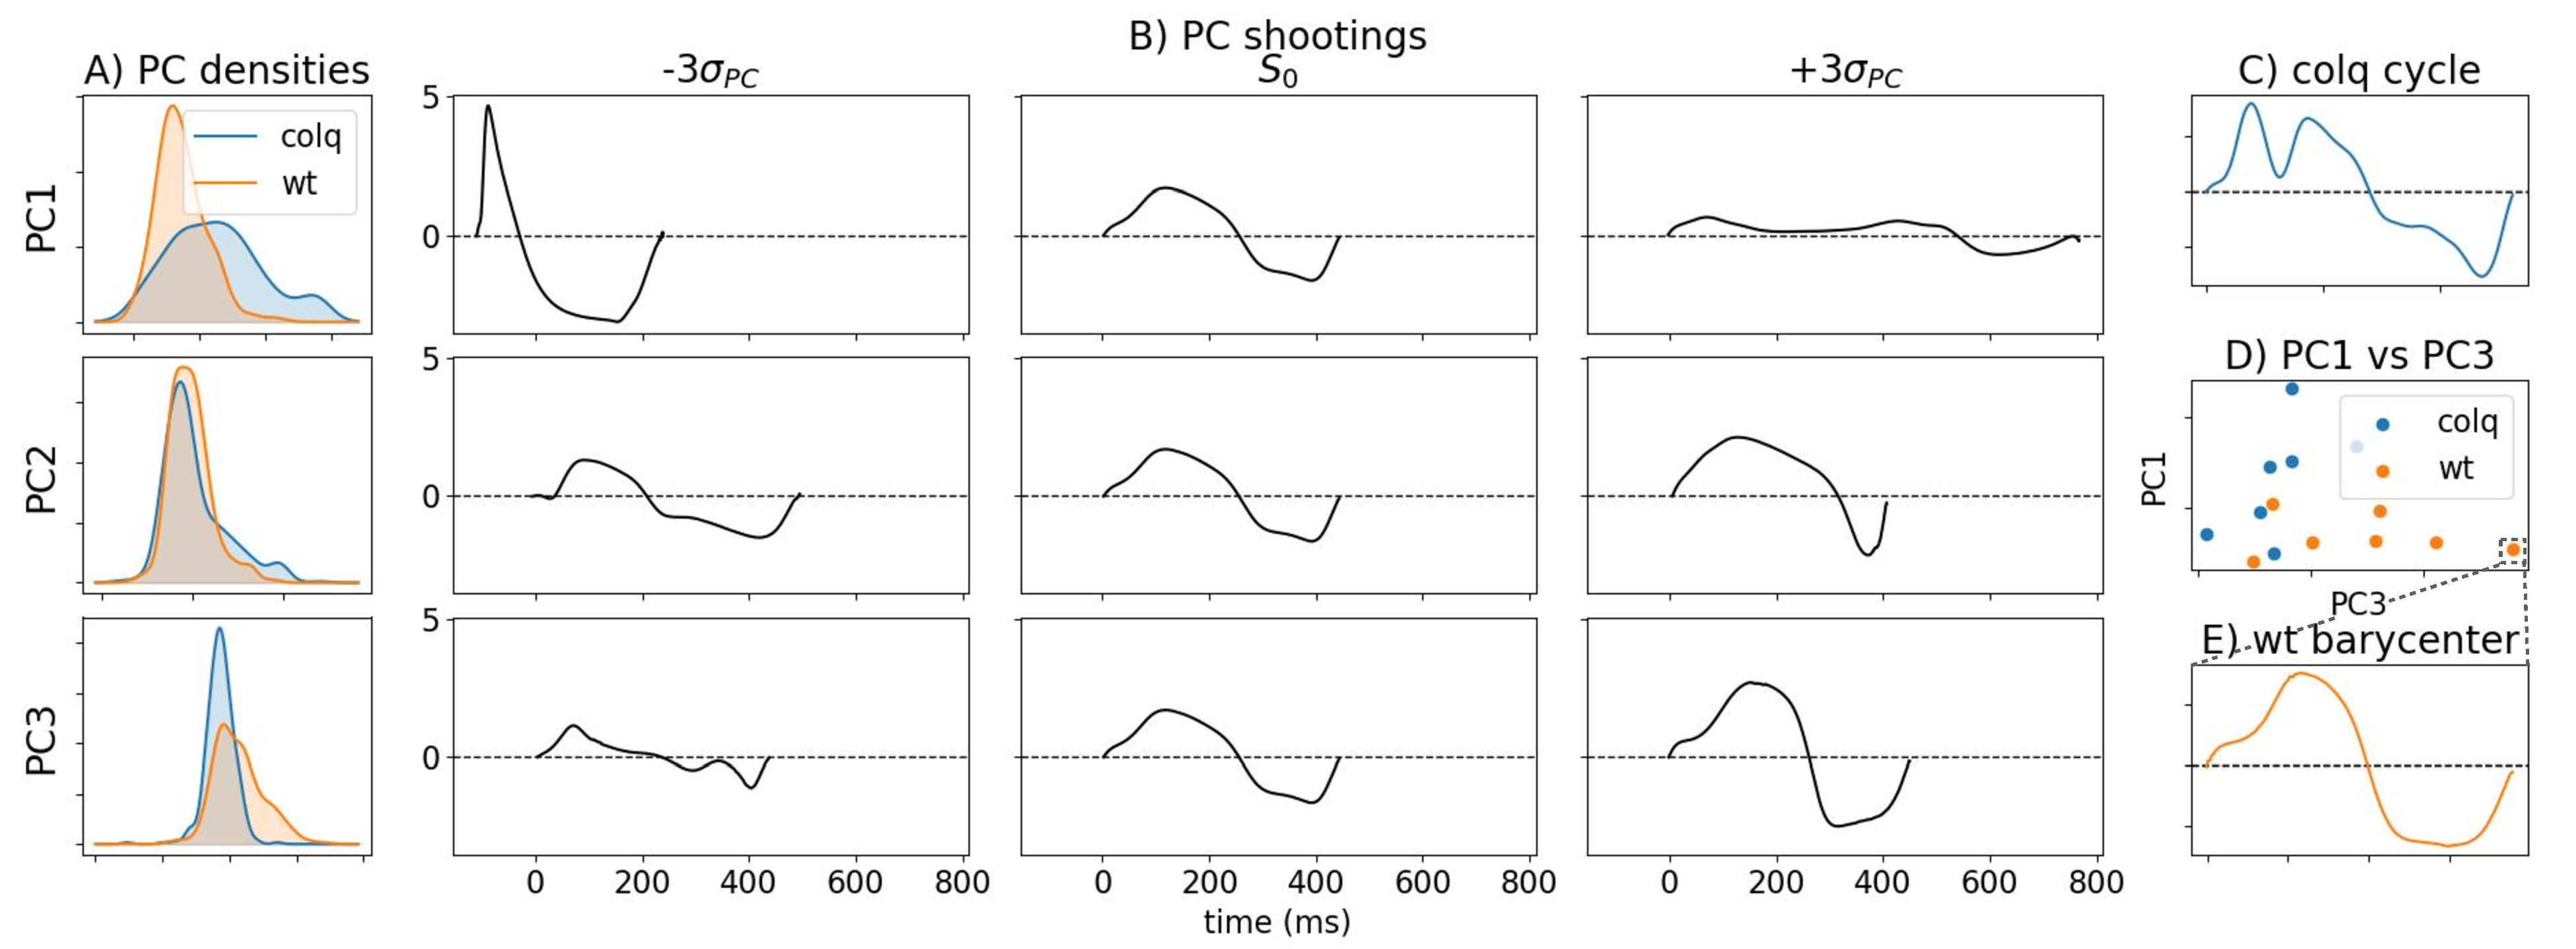
\includegraphics[width=0.95\linewidth]{"./pictures/exp_1_bis.pdf"}
%  \vspace{-1.5em}
%  \caption{Analysis of the two principal components (PC) related to the mice respiratory cycles before exposure for TS-LDDMM \Cref{fig:ts-lddmm shooting}.
%  In Figure A), the densities of each genotype according to each PC are displayed. In Figure B), the deformations of the reference graph $S_0$ along each PC are given. In Figure D), the graph of reference $S^j$, also called barycenter, related to each mouse, is displayed according to their coordinates on PC1 and PC3. In Figure C) et E), illustrations of respiratory cycles related to mice coming from the \textbf{wt} and \textbf{colq} group are displayed.  }
%  \label{fig:exp_1_PCA}
%  %\vspace{-1em}
%\end{figure*}

This experiment highlights the \textit{interpretability} of TS-LDDMM representation for studying the inter-individual variability in time series biomedical datasets. We consider a multivariate time series dataset that accounts for mice's nasal and thoracic airflow evolution when exposed to an irritant molecule altering respiratory functions \cite{nervo2019respiratory}.
The dataset is divided into two groups, one composed of 7 control mice (\textbf{wt}) and the other of 7 mice (\textbf{colq}) deficient in an enzyme involved in the control of respiration. For each mouse, airflows were recorded for 15 to 20 minutes before exposure to the irritant molecule and then for 35 to 40 minutes. A complete 
description of the dataset is given in the \Cref{appendix:mouse_dataset}.

\paragraph{Protocol.} For both experiments and representations (TS-LDDMM and LDDMM), we derive the reference respiratory cycle's graph $S_0$ and the representations $(\alpha_j)_{j\in[N]}$ related to $N$ respiratory cycles extracted according to the procedure \cite{germain2023unsupervised} by solving  \eqref{eq:general_optimization_problem}.
 Then, we perform a kernel PCA on the initial velocity field $\left(v_0(\alpha_j,S_0)\right)_{j\in[N]}\in \msv^{N_1}$ defined in \eqref{eq:def_v0} to breathing behavior.
  The first experiment includes $N_1 = 700$ respiratory cycles collected before exposure. The second experiment includes $N_2 = 1400$ respiratory cycles with 25\% (resp. 75\%) before (resp. after) exposure.
   \Cref{appendix: mice_exp_setting} describes methods settings.
    Essentially, varifold losses are identical for both methods, and the velocity field kernels are set to encompass time and space scales. 
    
    \vspace{-1ex}
\paragraph{Breathing behaviors before exposure.}
 We focus on the analysis of the two first Principal Components (PC) for TS-LDDMM (\Cref{fig:ts-lddmm shooting}), and LDDMM (\Cref{fig:lddmm shooting}).
  A respiratory cycle is an inspiration (positive flow) followed by an expiration (negative flow); \Cref{fig:wt-reference} displays an example of \textbf{wt} mouse respiratory cycle.
   \Cref{fig:exp1} shows that principal components learned with TS-LDMM lead to deformations that remain respiratory cycles, while deformations learned with LDDMM are challenging to interpret as respiratory cycles.
   The LDDMM velocity field kernel is a Gaussian anisotropic kernel that accounts for time and space scales; however, the entanglement of time and space dimensions in the kernel does not guarantee the graph structure, and it makes the convergence of the method difficult (relative varifold loss error: TS-LDDMM: 0.06, LDDMM: 0.11).
    Regarding TS-LDDMM, \Cref{fig:ts-lddmm shooting} shows its principal components refer to different types of deformations.
     By interpreting \Cref{fig:ts-lddmm shooting}: PC1 accounts for time warping, PC2 expresses the trade-off between inspiration and expiration duration.
      Compared to \textbf{wt} mice, the distribution of \textbf{colq} mice feature along the PC1 axis has a heavy left tail, and the associated deformation (-2 $\sigma_{\text{PC}}$) shows an inspiration with two peaks.
       \Cref{fig:colq-cycle} shows an example of such respiratory cycles, which may be caused by motor impairment due to enzyme deficiency \cite{germain2023unsupervised}.
        Finally, \Cref{fig: pcs-scatter} shows that PC1 and PC2 capture the main differences between the two groups as their respective reference graphs $S^j$ are located in different parts of the space. 

\begin{figure*}[t]
  \centering
  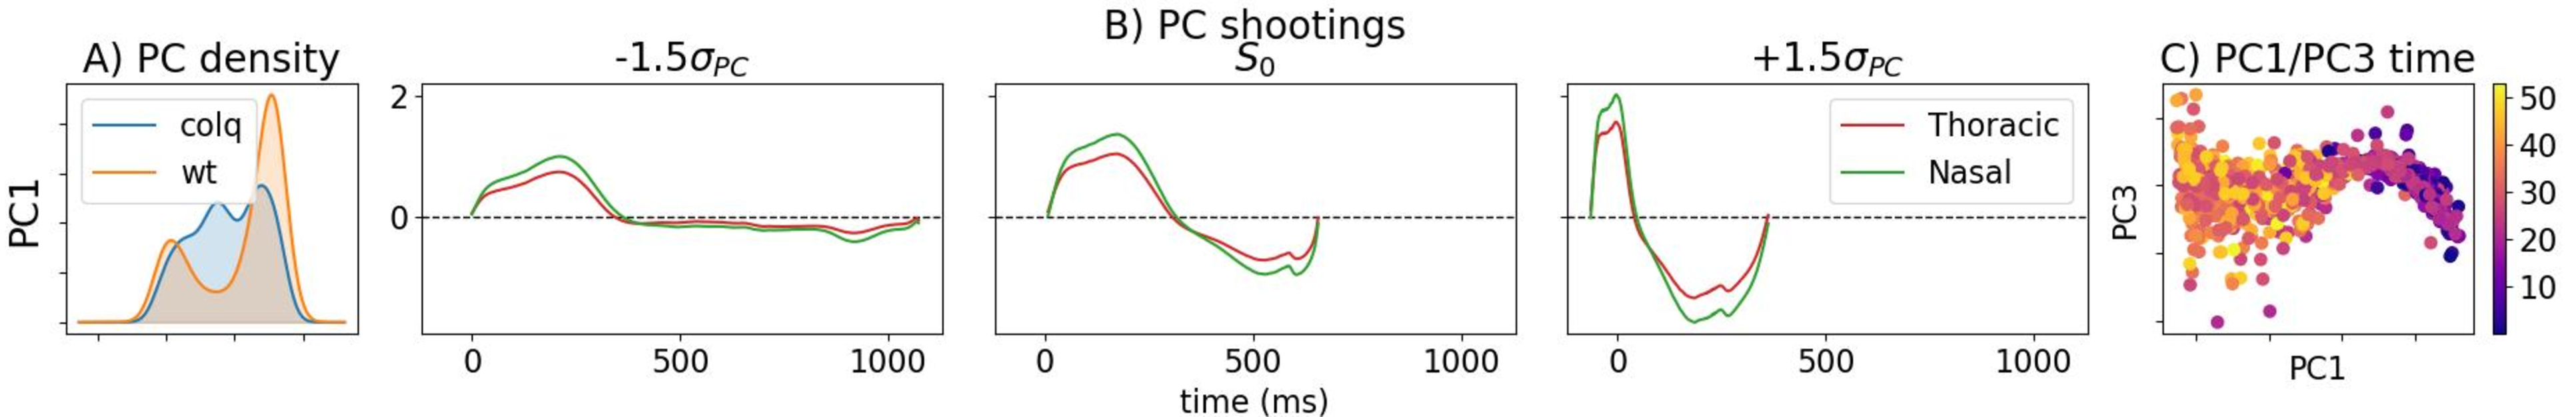
\includegraphics[width=0.95\linewidth]{"./pictures/exp2.pdf"}
  \caption{Analysis of the first Principal Component (PC1) related to mice' respiratory cycles before and after exposure for TS-LDDMM. Figure A) displays PC densities according to mice genotype, Figure B) displays  deformations of the reference graph $S_0$ along PC1, and Figure C) displays respiratory cycles with respect to time in PC1 and PC3 coordinates}
  \label{fig:exp_2_PCA}
  \vspace{-1.5em}
\end{figure*}
\vspace{-1ex}
\paragraph{Breathing behaviors' evolution after exposure to the irritant molecule} 
TS-LDDMM representation features are learned on a dataset that includes respiratory cycles before and after exposure.
 \Cref{fig:exp_2_PCA} displays the first principal component PC since it encodes the effect of the irritant molecule as depicted in \Cref{fig:exp_2_PCA}-C) (the exposure occurs at 20 minutes). \Cref{fig:exp_2_PCA}-B) shows that the deformation (-1.5 $\sigma_{\text{PC}}$) leads to longer respiratory cycles that include a pause between inspiration and expiration as observed in \cite{germain2023unsupervised}.
  Conjointly, \Cref{fig:exp_2_PCA}-A) shows a bimodal distribution for \textbf{wt} mice whereas \textbf{wt}' distributions before exposure were unimodal (\Cref{fig:ts-lddmm shooting}). Indeed, the irritant molecule inhibits the action of the deficient enzyme, \textbf{wt} mice strongly react to the irritant molecule, whereas \textbf{colq} mice better adapt due to their deficiency \cite{germain2023unsupervised}.
%   \vspace{-1ex}
% \paragraph{Result summary.} By comparing the shape of individual respiratory cycles, we show that TS-LDDMM features can encode genotype distinctive breathing behaviors and their evolution after exposure to the irritant molecule contrary to LDDMM \cite{glaunes2008large}. 
% \vspace{-1ex}
%Secondly, we compare breathing behaviors before and after exposure to observe the impact of the irritant molecule.
% We follow the same procedure as for before exposure, but we take $N_2=1400$ respiratory cycles extracted according 
% to the procedure CITE....
% In \Cref{fig:exp_2_PCA}, we focus on the first Principal Component (PC) since it encodes the effect of the irritant molecule as demonstrated on Figure \ref{fig:exp_2_PCA}-C) (exposure at time 20).
% We observe on \Cref{fig:exp_2_PCA}-B) that after exposure the mouse have longuer breath such that the expiration is longuer than inspiration.
%  Moreover, we deduce from Figure \ref{fig:exp_2_PCA}-A) that \textbf{colq} are more constant in their breath compared to \textbf{wt} after exposure.
%
% In Figure REF, we 
% also display the reference respiratory cycle S0 and its deformations in the principal component directions.
%  Additionally, we learn each mouse's reference respiratory cycle and represent them in the first and third PC coordinates system in Figure REF. 